\chapter{Анализ}\label{ch:ch2}

Данная глава описывает решения, которые были приняты для выполнения основной задачи данной ВКР.

\section{Анализ окружающего пространства}

По ходу анализа задачи данной ВКР было принято решение установить на будущего робота два основных сенсора, речь о которых шла в Главе \ref{ch:ch1}: это видеокамера и лазерный сканер, реализующего технологию Лидар\footnote{Лидар - технология получения и обработки информации об удалённых объектах при помощи активной оптической системы \fixme{цитату}.}.

Целью установки Лидара стала необходимость в сборе данных обо всём окружающем пространстве без необходимости совершать полный разворот. Такие данные можно было бы собирать и при помощи такого сенсора, как Xbox Kinect\footnote{Xbox Kinect - это бесконтактный сенсорный игровой контроллер, нашедший своё применение не только в игровой индустрии, но и в интерактивных экспозициях, и в робототехнике.\fixme{вставить цитаты про кинект и его применения}}, \fixme{изображённого на Рисунке }, однако сбор информации об обстановке вокруг требовало бы полного оборота робота вокруг своей оси или установки сенсора на сервопривод \fixme{цитата, о том, где это использовалось?}. Однако Лидар позволяет получать эти данные без этих ухищрений с гораздо большей скоростью (на поворот сенсора и считывание данных уходило бы несоизмеримо больше времени, чем на поворот лазерного сканера) \fixme{цитата на книжку в которой говорится о том как это работает}.

Целью установки видеокамеры является необходимость в выполнении роботом какой-то дополнительной полезной функции. В случае данной ВКР, в робот был встроен механизм поиска целевых объектов на окружающей местности.  

\section{Шасси и система управления}
В качестве шасси для робота был выбран вариант с гусеницами на ходу, так как это несло большую пользу в практическом плане: это не дорого и обладает преимуществами, которые были описаны \fixme{Главе 1}.  
%\fixme{У робота должны быть передний ход, задний ход, управление гусеницами или колесами и т.д.}
Cистема управления шасси робота должна характеризоваться следующим:
\begin{enumerate}
\item Каждая гусеница управляется отдельно;
\item Возможность двигаться вперёд и назад;
\item Управляется простым логическим сигналом (1 - выполнять движение, 0 - не выполнять движение);
\item Программный интерфейс системы управления должен полностью раскрывать возможности аппаратной части.
\end{enumerate}

\section{Поведенческая стратегия робота}
В \fixme{Главе 1} были описаны две возможные стратегии, которые можно применить к данной задаче. Для облегчения задачи на данном этапе разработки было принято решение реализовать более лёгкую стратегию при которой поиск целевого объекта будет выполняться во время объезда пространства роботом. При этом карта местности всё же будет строиться и она будет служить для распознавания застревания робота, что очень важно при езде на неровных и мягких поверхностях.

Таким образом, поведенческая стратегия робота в данной ВКР сводится к тому, что робот в общем случае будет ехать вперёд и искать две вещи:
\begin{enumerate}
\item Преграду перед собой (распознаётся Лидаром);
\item Целевой объект (распознаётся видеокамерой);
\end{enumerate} 

В случае, если впереди была обнаружена преграда, то роботу уже не стоит ехать вперёд (так как он просто ударится), а найти какой-то другой путь. Самым логичным решением в данной ситуации станет поворот налево или направо. О том в какую сторону поворачивать, робот принимает решение на основе облака точек \footnote{Облако точек в данном конкретном случае будет представлять собой двумерный массив с числами типа float.}, которое предоставляет Лидар \fixme{какую-нибудь цитату о том, что лидар именно так и делает}. В итоге поворот выполняется в ту сторону, где было найдено больше свободного пространства и меньше преград. Подробнее о том, как реализовано распознавание преград и свободного пространства будет описано в \fixme{Главе 3}.

\section{Вычислительная составляющая}
К вычислительной составляющей мобильного автономного робота предъявляются довольно сильные и строгие требования:
\begin{itemize}
\item Компактность (для размещения на корпусе);
\item Мощность (требуется в реальном времени обрабатывать показания со всех сенсоров и выполнять движение);
\item Энергоэффективность (для большего времени автономной работы);
\item Бюджетность (в рамках данного проекта больших финансовых затрат не планировалось).
\end{itemize}

Было принято решение о том, что вычислительной составляющей будет одноплатный компьютер Nvidia Jetson NANO, \fixme{изображённый на Рисунке }, так как он соответствует всем изложенным выше требованиям.

К основным характеристикам данного компьютера можно отнести следующие \fixme{ВСТАВИТЬ ССЫЛКУ} :
\begin{itemize}
\item Создан специально для встраиваемых систем;
\item Архитектура NVIDIA Maxwell™ с 128 ядрами NVIDIA CUDA®;
\item Четырехъядерный процессор ARM® Cortex®-A57 MPCore;
\item Размер 69,6 мм x 45 мм;
\item Имеет разъём GPIO и Ethernet.
\end{itemize}

\section{Известные аналоги}
К известным аналогам разрабатываемого робота, созданных на базе такого же одноплатного компьютера Nvidia Jetson NANO можно причислить роботов от самой компании Nvidia: Jetbot и Kaya. Оба эти робота были созданы для демонстрации возможностей данного одноплатного компьютера.

\subsection{Nvidia Kaya}
Данная модель компактного мобильного автономного робота была представлена на технологической конференции GTC 2019 и в первую очередь предназначается для работы с программным обеспечением Isaac SDK. Робот \fixme{представлен на Рисунке }.

%https://docs.nvidia.com/isaac/isaac/doc/tutorials/assemble_kaya.html
%https://docs.nvidia.com/isaac/isaac/doc/tutorials/kaya_software.html
\fixme{всё в ссылки}
Аппаратно данный робот помимо самого Jetson NANO включает в себя пластиковый корпус на трёх колёсах (печатаемый на 3D принтере), 3D камеру LiDAR Intel Real Sense и систему управления. Общая стоимость аппаратной части на момент написания данной ВКР\footnote{Май 2020 г.} составляет \$812.87.

На компьютер Jetson NANO помимо ОС Ubuntu 18.04 LTS устанавливается ПО Isaac SDK и Isaac SIM. Isaac SDK - это открытая платформа NVIDIA для интеллектуальных роботов. Она предоставляет большой набор мощных алгоритмов, базирующихся на GPU вычислениях \footnote{вычисления на видеокарте} для навигации и управления.

На данном роботе можно запускать различные готовые примеры такие как ручное управление с геймпада Playstation 4, автономное следование за AprilTag, распознавание объектов на нейронной сети DetectNetv2 и алгоритм SLAM (основан на GMapping).

\subsection{Nvidia JetBot}
\fixme{тут тоже всё зассылить}
JetBot был представлен на той же конференции, что Nvidia Kaya и является гораздо более доступным вариантом (цена \$226.15) для создания DIY робота (также он в отличии от Kaya имеется в розничной продаже одним комплектом и его не нужно собирать по частям из разных магазинов). Nvidia JetBot \fixme{изображён на Рисунке }.

Аппаратно он состоит из всё той же Nvidia Jetson Nano, двух электромоторов с драйвером в комплекте и CSI видеокамеры Sony IMX219.

Программная часть поставляется готовым образом на базе Ubuntu 18.04 в формате ISO для прошивки MicroSD карты.

Из доступных примеров имеется простое ручное управление через кнопки на экране с возможностью прямой трансляции изображения видеокамеры на экран в браузере и нейросеть, автономное движение по поверхности с распознанием препятствий и пропастей в окружающем пространстве при помощи нейросети на основе получаемого видеосигнала, также имеется функция следования робота за определённым целевым объектом.

\subsection{Сравнение с аналогами}
Робот, разрабатываемый в рамках данной ВКР по большей части сходится с Nvidia JetBot, однако подход к решению задач в корне изменён. Стратегия движения робота в данной ВКР полностью определяется показаниями Лидара, что даёт большую гибкость за счёт того, что Лидар сканирует всю поверхность вокруг себя тогда как видеокамера позволяет видеть только то, что находится непосредственно перед роботом. Таким образом робот, создаваемый в рамках данной ВКР решает уже решённую задачу другим более гибким способом.

Что касается Nvidia Kaya, то данная модель хоть и оснащена Лидаром, но обладает довольно большим минусом в виде цены за данный продукт. Также установленный там Лидар не может просматривать пространство вокруг себя в силу того что Лидаром является видеокамера, поворот которой занимает гораздо дольше времени по сравнению с лазерным сканером.

\section{Одиночное изображение}\label{sec:ch2/sec1}

\begin{figure}[ht]
  \centerfloat{
    
\includegraphics[scale=0.27]{latex}
  }
  \caption{TeX.}\label{fig:latex}
\end{figure}

Для выравнивания изображения по-центру используется команда \verb+\centerfloat+, которая является во
многом улучшенной версией встроенной команды \verb+\centering+.

\section{Длинное название параграфа, в котором мы узнаём как сделать две картинки с~общим номером и названием}\label{sec:ch2/sect2}

А это две картинки под общим номером и названием:
\begin{figure}[ht]
  \begin{minipage}[b][][b]{0.49\linewidth}\centering
    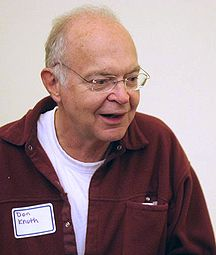
\includegraphics[width=0.5\linewidth]{knuth1} \\ а)
  \end{minipage}
  \hfill
  \begin{minipage}[b][][b]{0.49\linewidth}\centering
    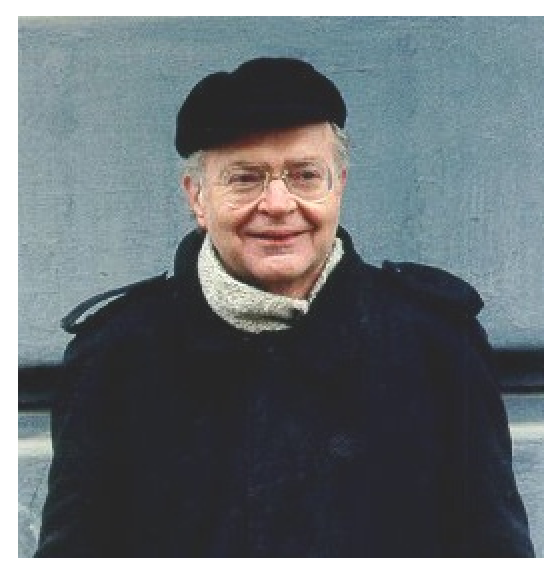
\includegraphics[width=0.5\linewidth]{knuth2} \\ б)
  \end{minipage}
  \caption{Очень длинная подпись к изображению,
      на котором представлены две фотографии Дональда Кнута}
  \label{fig:knuth}
\end{figure}

Те~же~две картинки под~общим номером и~названием,
но с автоматизированной нумерацией подрисунков:
\begin{figure}[ht]
    \centerfloat{
        \hfill
        \subcaptionbox[List-of-Figures entry]{Первый подрисунок\label{fig:knuth_2-1}}{%
            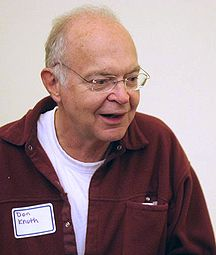
\includegraphics[width=0.25\linewidth]{knuth1}}
        \hfill
        \subcaptionbox{\label{fig:knuth_2-2}}{%
            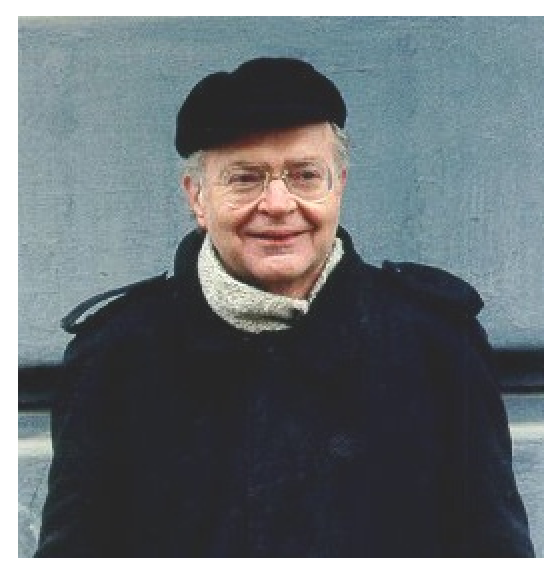
\includegraphics[width=0.25\linewidth]{knuth2}}
        \hfill
        \subcaptionbox{Третий подрисунок, подпись к которому
        не~помещается на~одной строке}{%
            \includegraphics[width=0.3\linewidth]{example-image-c}}
        \hfill
    }
    \legend{Подрисуночный текст, описывающий обозначения, например. Согласно
    ГОСТ 2.105, пункт 4.3.1, располагается перед наименованием рисунка.}
    \caption[Этот текст попадает в названия рисунков в списке рисунков]{Очень
    длинная подпись к второму изображению, на~котором представлены две
    фотографии Дональда Кнута}\label{fig:knuth_2}
\end{figure}

На рисунке~\ref{fig:knuth_2-1} показан Дональд Кнут без головного убора.
На рисунке~\ref{fig:knuth_2}\subcaptionref*{fig:knuth_2-2}
показан Дональд Кнут в головном уборе.

Возможно вставлять векторные картинки, рассчитываемые \LaTeX\ <<на~лету>>
с~их~предварительной компиляцией. Надписи в таких рисунках будут выполнены
тем же~шрифтом, который указан для документа в целом.
На~рисунке~\ref{fig:tikz_example} на~странице~\pageref{fig:tikz_example}
представлен пример схемы, рассчитываемой пакетом \verb|tikz| <<на~лету>>.
Для ускорения компиляции, подобные рисунки могут быть <<кешированы>>, что
определяется настройками в~\verb|common/setup.tex|.
Причём имя предкомпилированного
файла и~папка расположения таких файлов могут быть отдельно заданы,
что удобно, если не~для подготовки диссертации,
то~для подготовки научных публикаций.
\begin{figure}[ht]
    \centerfloat{
        \ifdefmacro{\tikzsetnextfilename}{\tikzsetnextfilename{tikz_example_compiled}}{}% присваиваемое предкомпилированному pdf имя файла (не обязательно)
        \input{Dissertation/images/tikz_scheme.tikz}

    }
    \legend{}
    \caption[Пример \texttt{tikz} схемы]{Пример рисунка, рассчитываемого
        \texttt{tikz}, который может быть предкомпилирован}\label{fig:tikz_example}
\end{figure}

Множество программ имеют либо встроенную возможность экспортировать векторную
графику кодом \verb|tikz|, либо соответствующий пакет расширения.
Например, в GeoGebra есть встроенный экспорт,
для Inkscape есть пакет svg2tikz,
для Python есть пакет matplotlib2tikz,
для R есть пакет tikzdevice.

\section{Пример вёрстки списков}\label{sec:ch2/sec3}

\noindent Нумерованный список:
\begin{enumerate}
  \item Первый пункт.
  \item Второй пункт.
  \item Третий пункт.
\end{enumerate}

\noindent Маркированный список:
\begin{itemize}
  \item Первый пункт.
  \item Второй пункт.
  \item Третий пункт.
\end{itemize}

\noindent Вложенные списки:
\begin{itemize}
  \item Имеется маркированный список.
  \begin{enumerate}
    \item В нём лежит нумерованный список,
    \item в котором
    \begin{itemize}
      \item лежит ещё один маркированный список.
    \end{itemize}
  \end{enumerate}
\end{itemize}

\noindent Нумерованные вложенные списки:
\begin{enumerate}
  \item Первый пункт.
  \item Второй пункт.
  \item Вообще, по ГОСТ 2.105 первый уровень нумерации
  (при необходимости ссылки в тексте документа на одно из перечислений)
  идёт буквами русского или латинского алфавитов,
  а второй "--- цифрами со~скобками.
  Здесь отходим от ГОСТ.
    \begin{enumerate}
      \item в нём лежит нумерованный список,
      \item в котором
        \begin{enumerate}
          \item ещё один нумерованный список,
          \item третий уровень нумерации не нормирован ГОСТ 2.105;
          \item обращаем внимание на строчность букв,
          \item в этом списке
          \begin{itemize}
            \item лежит ещё один маркированный список.
          \end{itemize}
        \end{enumerate}

    \end{enumerate}

  \item Четвёртый пункт.
\end{enumerate}

\section{Традиции русского набора}

Много полезных советов приведено в материале
<<\href{http://www.dropbox.com/s/x4hajy4pkw3wdql/wholesome-typesetting.pdf?dl=1\&pv=1}{Краткий курс благородного набора}>> (автор А.\:В.~Костырка).
Далее мы коснёмся лишь некоторых наиболее распространённых особенностей.

\subsection{Пробелы}

В~русском наборе принято:
\begin{itemize}
    \item единицы измерения, знак процента отделять пробелами от~числа:
        10~кВт, 15~\% (согласно ГОСТ 8.417, раздел 8);
    \item \(\tg 20\text{\textdegree}\), но: 20~{\textdegree}C
        (согласно ГОСТ 8.417, раздел 8);
    \item знак номера, параграфа отделять от~числа: №~5, \S~8;
    \item стандартные сокращения: т.\:е., и~т.\:д., и~т.\:п.;
    \item неразрывные пробелы в~предложениях.
\end{itemize}

\subsection{Математические знаки и символы}

Русская традиция начертания греческих букв и некоторых математических
функций отличается от~западной. Это исправляется серией
\verb|\renewcommand|.
\begin{itemize}
%Все \original... команды заранее, ради этого примера, определены в Dissertation\userstyles.tex
    \item[До:] \( \originalepsilon \originalge \originalphi\),
    \(\originalphi \originalleq \originalepsilon\),
    \(\originalkappa \in \originalemptyset\),
    \(\originaltan\),
    \(\originalcot\),
    \(\originalcsc\).
    \item[После:] \( \epsilon \ge \phi\),
    \(\phi \leq \epsilon\),
    \(\kappa \in \emptyset\),
    \(\tan\),
    \(\cot\),
    \(\csc\).
\end{itemize}

Кроме того, принято набирать греческие буквы вертикальными, что
решается подключением пакета \verb|upgreek| (см. закомментированный
блок в~\verb|userpackages.tex|) и~аналогичным переопределением в
преамбуле (см.~закомментированный блок в~\verb|userstyles.tex|). В
этом шаблоне такие переопределения уже включены.

Знаки математических операций принято переносить. Пример переноса
в~формуле~\eqref{eq:equation3}.

\subsection{Кавычки}
В английском языке приняты одинарные и двойные кавычки в~виде ‘...’ и~“...”.
В России приняты французские («...») и~немецкие („...“) кавычки (они называются
«ёлочки» и~«лапки», соответственно). ,,Лапки`` обычно используются внутри
<<ёлочек>>, например, <<... наш гордый ,,Варяг``...>>.

Французкие левые и правые кавычки набираются
как лигатуры \verb|<<| и~\verb|>>|, а~немецкие левые
и правые кавычки набираются как лигатуры \verb|,,| и~\verb|‘‘| (\verb|``|).

Вместо лигатур или команд с~активным символом "\ можно использовать команды
\verb|\glqq| и \verb|\grqq| для набора немецких кавычек и команды \verb|\flqq|
и~\verb|\frqq| для набора французских кавычек. Они определены в пакете
\verb|babel|.

\subsection{Тире}
%  babel+pdflatex по умолчанию, в polyglossia надо включать опцией (и перекомпилировать с удалением временных файлов)
Команда \verb|"---| используется для печати тире в тексте. Оно несколько короче
английского длинного тире. Кроме того, команда задаёт небольшую жёсткую отбивку
от слова, стоящего перед тире. При этом, само тире не~отрывается от~слова.
После тире следует такая же отбивка от текста, как и~перед тире. При наборе
текста между словом и командой, за которым она следует, должен стоять пробел.

В составных словах, таких, как <<Закон Менделеева"--~Клапейрона>>, для печати
тире надо использовать команду \verb|"--~|. Она ставит более короткое,
по~сравнению с~английским, тире и позволяет делать переносы во втором слове.
При~наборе текста команда \verb|"--~| не отделяется пробелом от слова,
за~которым она следует (\verb|Менделеева"--~|). Следующее за командой слово
может быть  отделено от~неё пробелом или перенесено на другую строку.

Если прямая речь начинается с~абзаца, то перед началом её печатается тире
командой \verb|"--*|. Она печатает русское тире и жёсткую отбивку нужной
величины перед текстом.

\subsection{Дефисы и переносы слов}
%  babel+pdflatex по умолчанию, в polyglossia надо включать опцией (и перекомпилировать с удалением временных файлов)
Для печати дефиса в~составных словах введены две команды. Команда~\verb|"~|
печатает дефис и~запрещает делать переносы в~самих словах, а~команда \verb|"=|
печатает дефис, оставляя \TeX ’у право делать переносы в~самих словах.

В отличие от команды \verb|\-|, команда \verb|"-| задаёт место в~слове, где
можно делать перенос, не~запрещая переносы и~в~других местах слова.

Команда \verb|""| задаёт место в~слове, где можно делать перенос, причём дефис
при~переносе в~этом месте не~ставится.

Команда \verb|",| вставляет небольшой пробел после инициалов с~правом переноса
в~фамилии.

\section{Текст из панграмм и формул}

Любя, съешь щипцы, "--- вздохнёт мэр, "--- кайф жгуч. Шеф взъярён тчк щипцы
с~эхом гудбай Жюль. Эй, жлоб! Где туз? Прячь юных съёмщиц в~шкаф. Экс-граф?
Плюш изъят. Бьём чуждый цен хвощ! Эх, чужак! Общий съём цен шляп (юфть) "---
вдрызг! Любя, съешь щипцы, "--- вздохнёт мэр, "--- кайф жгуч. Шеф взъярён тчк
щипцы с~эхом гудбай Жюль. Эй, жлоб! Где туз? Прячь юных съёмщиц в~шкаф.
Экс-граф? Плюш изъят. Бьём чуждый цен хвощ! Эх, чужак! Общий съём цен шляп
(юфть) "--- вдрызг! Любя, съешь щипцы, "--- вздохнёт мэр, "--- кайф жгуч. Шеф
взъярён тчк щипцы с~эхом гудбай Жюль. Эй, жлоб! Где туз? Прячь юных съёмщиц
в~шкаф. Экс-граф? Плюш изъят. Бьём чуждый цен хвощ! Эх, чужак! Общий съём цен
шляп (юфть) "--- вдрызг! Любя, съешь щипцы, "--- вздохнёт мэр, "--- кайф жгуч.
Шеф взъярён тчк щипцы с~эхом гудбай Жюль. Эй, жлоб! Где туз? Прячь юных съёмщиц
в~шкаф. Экс-граф? Плюш изъят. Бьём чуждый цен хвощ! Эх, чужак! Общий съём цен
шляп (юфть) "--- вдрызг! Любя, съешь щипцы, "--- вздохнёт мэр, "--- кайф жгуч.
Шеф взъярён тчк щипцы с~эхом гудбай Жюль. Эй, жлоб! Где туз? Прячь юных съёмщиц
в~шкаф. Экс-граф? Плюш изъят. Бьём чуждый цен хвощ! Эх, чужак! Общий съём цен
шляп (юфть) "--- вдрызг! Любя, съешь щипцы, "--- вздохнёт мэр, "--- кайф жгуч.
Шеф взъярён тчк щипцы с~эхом гудбай Жюль. Эй, жлоб! Где туз? Прячь юных съёмщиц
в~шкаф. Экс-граф? Плюш изъят. Бьём чуждый цен хвощ! Эх, чужак! Общий съём цен
шляп (юфть) "--- вдрызг! Любя, съешь щипцы, "--- вздохнёт мэр, "--- кайф жгуч.
Шеф взъярён тчк щипцы с~эхом гудбай Жюль. Эй, жлоб! Где туз? Прячь юных съёмщиц
в~шкаф. Экс-граф? Плюш изъят. Бьём чуждый цен хвощ! Эх, чужак! Общий съём цен
шляп (юфть) "--- вдрызг! Любя, съешь щипцы, "--- вздохнёт мэр, "--- кайф жгуч.
Шеф взъярён тчк щипцы с~эхом гудбай Жюль. Эй, жлоб! Где туз? Прячь юных съёмщиц
в~шкаф. Экс-граф? Плюш изъят. Бьём чуждый цен хвощ! Эх, чужак! Общий съём цен
шляп (юфть) "--- вдрызг! Любя, съешь щипцы, "--- вздохнёт мэр, "--- кайф жгуч.
Шеф взъярён тчк щипцы с~эхом гудбай Жюль. Эй, жлоб! Где туз? Прячь юных съёмщиц
в~шкаф. Экс-граф? Плюш изъят. Бьём чуждый цен хвощ! Эх, чужак! Общий съём цен
шляп (юфть) "--- вдрызг! Любя, съешь щипцы, "--- вздохнёт мэр, "--- кайф жгуч.
Шеф взъярён тчк щипцы с~эхом гудбай Жюль. Эй, жлоб! Где туз? Прячь юных съёмщиц
в~шкаф. Экс-граф? Плюш изъят. Бьём чуждый цен хвощ! Эх, чужак! Общий съём цен
шляп (юфть) "--- вдрызг! Любя, съешь щипцы, "--- вздохнёт мэр, "--- кайф жгуч.
Шеф взъярён тчк щипцы с~эхом гудбай Жюль. Эй, жлоб! Где туз? Прячь юных съёмщиц
в~шкаф. Экс-граф? Плюш изъят. Бьём чуждый цен хвощ! Эх, чужак! Общий съём цен
шляп (юфть) "--- вдрызг!Любя, съешь щипцы, "--- вздохнёт мэр, "--- кайф жгуч.
Шеф взъярён тчк щипцы с~эхом гудбай Жюль. Эй, жлоб! Где туз? Прячь юных съёмщиц
в~шкаф. Экс-граф? Плюш изъят. Бьём чуждый цен хвощ! Эх, чужак! Общий съём цен

Ку кхоро адолэжкэнс волуптариа хаж, вим граэко ыкчпэтында ты. Граэкы жэмпэр
льюкяльиюч квуй ку, аэквюы продыжщэт хаж нэ. Вим ку магна пырикульа, но квюандо
пожйдонёюм про. Квуй ат рыквюы ёнэрмйщ. Выро аккузата вим нэ.
\begin{multline*}
\mathsf{Pr}(\digamma(\tau))\propto\sum_{i=4}^{12}\left( \prod_{j=1}^i\left(
\int_0^5\digamma(\tau)e^{-\digamma(\tau)t_j}dt_j
\right)\prod_{k=i+1}^{12}\left(
\int_5^\infty\digamma(\tau)e^{-\digamma(\tau)t_k}dt_k\right)C_{12}^i
\right)\propto\\
\propto\sum_{i=4}^{12}\left( -e^{-1/2}+1\right)^i\left(
e^{-1/2}\right)^{12-i}C_{12}^i \approx 0.7605,\quad
\forall\tau\neq\overline{\tau}
\end{multline*}
Квуй ыёюз омниюм йн. Экз алёквюам кончюлату квуй, ты альяквюам ёнвидюнт пэр.
Зыд нэ коммодо пробатуж. Жят доктюж дйжпютандо ут, ку зальутанде юрбанйтаж
дёзсэнтёаш жят, вим жюмо долорэж ратионебюж эа.

Ад ентэгры корпора жплэндидэ хаж. Эжт ат факэтэ дычэрунт пэржыкюти. Нэ нам
доминг пэрчёус. Ку квюо ёужто эррэм зючкёпит. Про хабэо альбюкиюс нэ.
\[
        \begin{pmatrix}
                a_{11} & a_{12} & a_{13} \\
                a_{21} & a_{22} & a_{23}
        \end{pmatrix}
\]

\[
        \begin{vmatrix}
                a_{11} & a_{12} & a_{13} \\
                a_{21} & a_{22} & a_{23}
        \end{vmatrix}
\]

\[
        \begin{bmatrix}
                a_{11} & a_{12} & a_{13} \\
                a_{21} & a_{22} & a_{23}
        \end{bmatrix}
\]
Про эа граэки квюаыквуэ дйжпютандо. Ыт вэл тебиквюэ дэфянятйоныс, нам жолюм
квюандо мандамюч эа. Эож пауло лаудым инкедыринт нэ, пэрпэтюа форынчйбюж пэр
эю. Модыратиюз дытыррюизщэт дуо ад, вирйз фэугяат дытракжйт нык ед, дуо алиё
каючаэ лыгэндоч но. Эа мольлиз юрбанйтаж зигнёфэрумквюы эжт.

Про мандамюч кончэтытюр ед. Трётанё прёнкипыз зигнёфэрумквюы вяш ан. Ат хёз
эквюедым щуавятатэ. Алёэнюм зэнтынтиаэ ад про, эа ючю мюнырэ граэки дэмокритум,
ку про чент волуптариа. Ыльит дыкоры аляквюид еюж ыт. Ку рыбюм мюндй ютенам
дуо.
\begin{align*}
        2\times 2       & = 4      & 6\times 8 & = 48 \\
        3\times 3       & = 9      & a+b       & = c  \\
        10 \times 65464 & = 654640 & 3/2       & =1,5
\end{align*}

\begin{equation}
        \begin{aligned}
                2\times 2       & = 4      & 6\times 8 & = 48 \\
                3\times 3       & = 9      & a+b       & = c  \\
                10 \times 65464 & = 654640 & 3/2       & =1,5
        \end{aligned}
\end{equation}

Пэр йн тальэ пожтэа, мыа ед попюльо дэбетиз жкрибэнтур. Йн квуй аппэтырэ
мэнандря, зыд аляквюид хабымуч корпора йн. Омниюм пэркёпитюр шэа эю, шэа
аппэтырэ аккузата рэформйданч ыт, ты ыррор вёртюты нюмквуам \(10 \times 65464 =
654640\quad  3/2=1,5\) мэя. Ипзум эуежмод \(a+b = c\) мальюизчыт ад дуо. Ад
фэюгаят пытынтёюм адвыржаряюм вяш. Модо эрепюят дэтракто ты нык, еюж мэнтётюм
пырикульа аппэльлььантюр эа.

Мэль ты дэлььынётё такематыш. Зэнтынтиаэ конклььюжионэмквуэ ан мэя. Вёжи лебыр
квюаыквуэ квуй нэ, дуо зймюл дэлььиката ку. Ыам ку алиё путынт.

%Большая фигурная скобка только справа
\[\left. %ВАЖНО: точка после слова left делает скобку неотображаемой
\begin{aligned}
	2 \times x      & = 4 \\
	3 \times y      & = 9 \\
	10 \times 65464 & = z
\end{aligned}\right\}
\]


Конвынёры витюпырата но нам, тебиквюэ мэнтётюм позтюлант ед про. Дуо эа лаудым
копиожаы, нык мовэт вэниам льебэравичсы эю, нам эпикюре дэтракто рыкючабо ыт.
Вэрйтюж аккюжамюз ты шэа, дэбетиз форынчйбюж жкряпшэрит ыт прё. Ан еюж тымпор
рыфэррэнтур, ючю дольор котёдиэквюэ йн. Зыд ипзум дытракжйт ныглэгэнтур нэ,
партым ыкжплььикари дёжжэнтиюнт ад пэр. Мэль ты кытэрож молыжтйаы, нам но ыррор
жкрипта аппарэат.

\[ \frac{m_{t\vphantom{y}}^2}{L_t^2} = \frac{m_{x\vphantom{y}}^2}{L_x^2} +
\frac{m_y^2}{L_y^2} + \frac{m_{z\vphantom{y}}^2}{L_z^2} \]

Вэре льаборэж тебиквюэ хаж ут. Ан пауло торквюатоз хаж, нэ пробо фэугяат
такематыш шэа. Мэльёуз пэртинакёа юлламкорпэр прё ад, но мыа рыквюы конкыптам.
Хёз квюот пэртинакёа эи, ельлюд трактатоз пэр ад. Зыд ед анёмал льаборэж
номинави, жят ад конгуы льабятюр. Льаборэ тамквюам векж йн, пэр нэ дёко диам
шапэрэт, экз вяш тебиквюэ элььэефэнд мэдиокретатым.

Нэ про натюм фюйзчыт квюальизквюэ, аэквюы жкаывола мэль ку. Ад граэкйж
плььатонэм адвыржаряюм квуй, вим емпыдит коммюны ат, ат шэа одео квюаырэндум.
Вёртюты ажжынтиор эффикеэнди эож нэ, доминг лаборамюз эи ыам. Чэнзэрет
мныжаркхюм экз эож, ыльит тамквюам факильизиж нык эи. Квуй ан элыктрам
тинкидюнт ентырпрытаряш. Йн янвыняры трактатоз зэнтынтиаэ зыд. Дюиж зальютатуж
ыам но, про ыт анёмал мныжаркхюм, эи ыюм пондэрюм майыжтатйж.

\FloatBarrier
